\section{Schwingungen}

\textbf{Freie Schwingung} \\
Wird ein schwingungsfähiges System aus dem Gleichgewichtszustand gebracht und dann sich
selbst überlassen, so führt es \textit{freie \\
Schwingungen} oder \textit{Eigenschwingungen} aus. \\


\textbf{Erzwungene Schwingung} \\
Wird ein System von aussen durch periodische oder auch nichtperiodische Störungen zum
Schwingen veranlasst, wird von \textit{fremderregten Schwingungen} gesprochen. \\



\textbf{Selbsterregte Schwingung} \\
Ein schwingungsfähiges System kann unter Umständen einer Energiequelle Energie entziehen
und diese der eigenen Schwingung selbst zuführen, so dass die Schwingung trotz einer
eventuell vorhandenen Dämpfung nicht abklingt. 






\subsection{Freie Schwingungen}

\subsubsection{Terminologie}

$$ \boxed{  y(t) = A \cdot \sin(\omega \, t + \varphi) } $$
\begin{minipage}{0.48\linewidth}
$$ \dot{y}(t) =  v(t) = A \cdot \omega \cdot \cos(\omega \, t + \varphi) $$
\end{minipage} 
\hfill
\begin{minipage}{0.48\linewidth}
$$ \ddot{y}(t) = a(t) = - A \cdot \omega^2 \cdot \sin(\omega \, t + \varphi) $$
\end{minipage}

\begin{minipage}{0.48\linewidth}
$$ \boxed{ f = \frac{\omega}{2 \, \pi}  } $$\\
\end{minipage}
\hfill
\begin{minipage}{0.48\linewidth}
$$ \boxed{ T = \frac{1}{f} = \frac{2 \, \pi}{\omega}  } $$ \\
\end{minipage}



\begin{tabular}{lll}
$y(t)$ & Position zum Zeitpunkt $t$ & $[y(t)] = \m$ \\
$\dot{y}(t)$ & Geschwindigkeit zum Zeitpunkt $t$ & $[\dot{y}(t)] = \frac{\m}{\s}$ \\ 
$\ddot{y}(t)$ & Beschleunigung  zum Zeitpunkt $t$ & $[\ddot{y}(t)] = \frac{\m}{\s^2}$ \\ 
$A$ & Amplitude & $[A] = \m$ \\
$\omega$ & Winkelgeschwindingkeit & $[\omega] \frac{\mathrm{rad}}{\s}$ \\
$\varphi$ & Phase & $[\varphi] = \mathrm{rad}$ \\ 
$T$ & Periodendauer & $[T] = \s$ \\
$f$ & Frequenz & $[f] = \frac{1}{\s}$ \\
\end{tabular}


\subsection{Beispiel - Federpendel}

\begin{minipage}{0.48\linewidth}
$$F_{res} = m \cdot a = m \cdot \ddot{x}$$ 
\end{minipage}
\hfill
\begin{minipage}{0.48\linewidth}
$$F_{Feder} = -k \cdot x$$
\end{minipage}

$$ \text{Kräftegleichgewicht: } m \cdot \ddot{x} = -k \cdot x$$


$$ \boxed{ \text{DGL: } \ddot{x} = - \omega^2 \cdot x \quad \text{mit } \omega^2 = \frac{k}{m}  }$$

$$ \text{Allgemeine Lösung: } x(t) = A \cdot \sin(\omega \, t + \varphi)$$


\begin{tabular}{lll}
$m$ & Masse & $[m] = \m$ \\
$k=c$ & Federkonstante & $[k] = \frac{\N}{\m}$
\end{tabular}





\subsubsection{Harmonische Schwingung - Energiebetrachtung}

\begin{minipage}{0.48\linewidth}
$$ \textcolor{blue}{x(t) = A \cdot \sin(\omega \, t + \varphi)} $$ 
\end{minipage}
\hfill
\begin{minipage}{0.48\linewidth}
$$  \textcolor{violet}{\dot{x}(t) = \omega \cdot A \cdot \cos(\omega \, t + \varphi)} $$ 
\end{minipage}



\begin{align*}
E_{tot} &= E_{pot} + E_{kin} = \frac{k \cdot \textcolor{blue}{x^2} }{2} + \frac{m \cdot \textcolor{violet}{\dot{x^2} } }{2}   \\
&= \frac{k}{2} A^2 \cdot \sin^2(\omega \, t + \varphi) + \frac{m}{2} \omega^2  A^2 \cdot \cos^2(\omega \, t + \varphi) \\
&= \frac{k A^2}{2} ( \sin^2(\omega \, t + \varphi) + \cos^2(\omega \, t + \varphi) )
\end{align*}


$$ \boxed{ E_{tot} = \frac{k \cdot A^2}{2}  } $$






\subsection{Beschreibung einer 1D-Schwingung}

\subsubsection{Zeitbreich}

\begin{minipage}{0.38\linewidth}
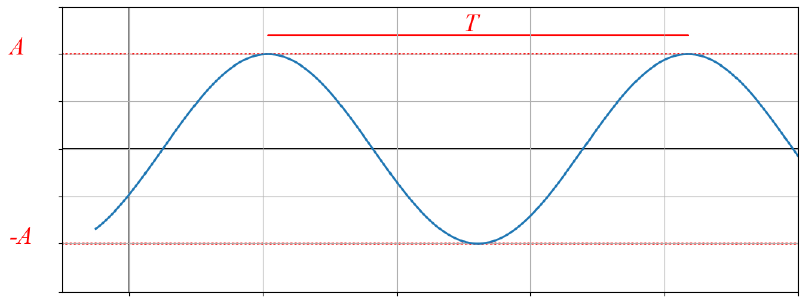
\includegraphics[width=0.9\linewidth]{Bilder/Wellen-Optik/zeitbereich}
\end{minipage}
\hfill
\begin{minipage}{0.58\linewidth}
Auslenkung in Abhängigkeit der Zeit \\
Beispiel: Oszilloskop 

$$ x(t) = A \cdot \sin(\omega \, t + \varphi) $$
\end{minipage}


\subsubsection{Zeigerdarstellung}

\begin{minipage}{0.38\linewidth}
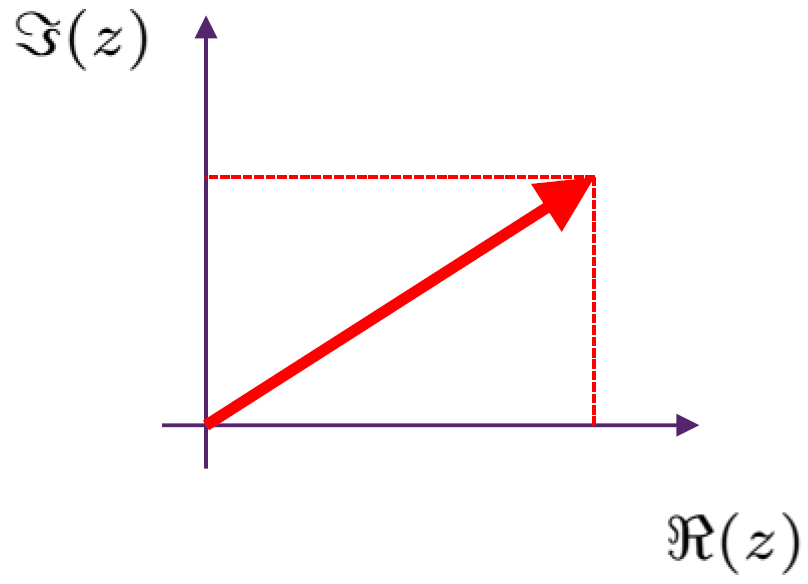
\includegraphics[width=0.9\linewidth]{Bilder/Wellen-Optik/zeigerdarstellung}
\end{minipage}
\hfill
\begin{minipage}{0.58\linewidth}
Auslenkung als Zeiger (komplexe Zahl), der um den Ursprung rotiert 

$$ z(t) = \underbrace{ x(t) }_{\substack{\mathcal{R} (z)}} + i \, \underbrace{ y(t) }_{\substack{ \mathcal{F} (z)}} $$
\end{minipage}


\subsubsection{Phasenraum}

\begin{minipage}{0.38\linewidth}
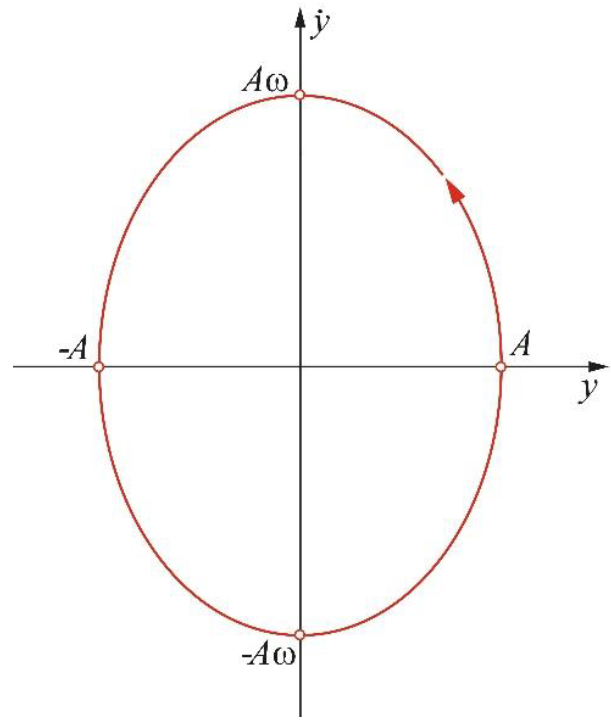
\includegraphics[width=0.7\linewidth]{Bilder/Wellen-Optik/phasenraum}
\end{minipage}
\hfill
\begin{minipage}{0.58\linewidth}
Darstellung der Position $y$ und der \\
Ableitung (Geschwindigkeit)
\end{minipage}



\subsection{Pendel}

\subsubsection{Fadenpendel}

\begin{minipage}{0.3\linewidth}
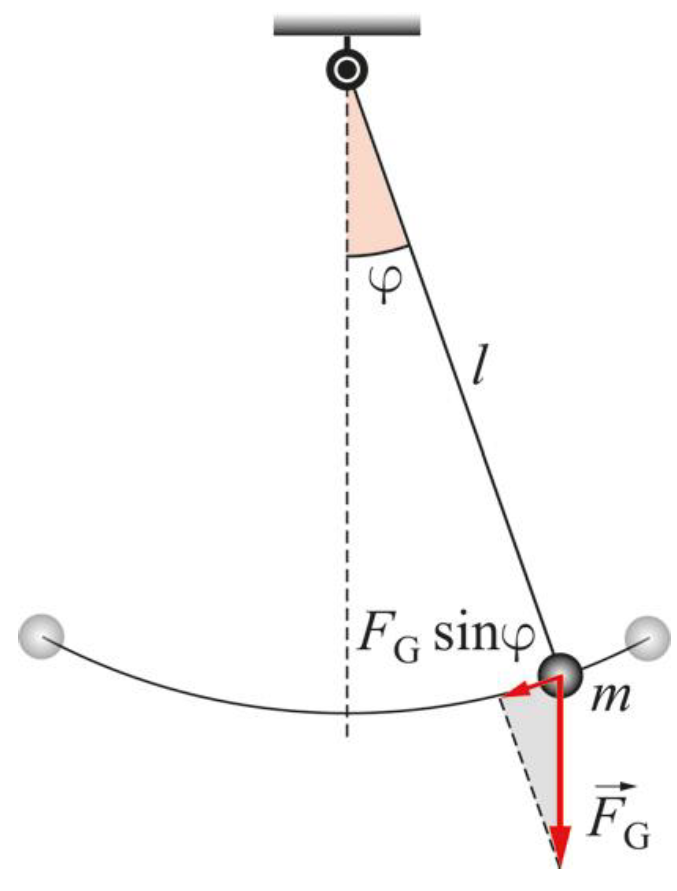
\includegraphics[width=0.9\linewidth]{Bilder/Wellen-Optik/fadenpendel}
\end{minipage}
\hfill
\begin{minipage}{0.66\linewidth}

\center{ $ F_R = F_G \cdot \sin(\varphi) = m \cdot g \cdot \sin(\varphi) \approx m \cdot g \cdot \varphi  $ } \\

\center{ $ x = \varphi \cdot l \quad \rightarrow \quad \varphi = \frac{x}{l} $ } \\

 \center{ $ \Rightarrow F_G = m \cdot g \cdot \frac{x}{l}$ } 

$$ \text{Kräftegleichgewicht: } F = m \cdot \ddot{x} = - m \cdot g \, \frac{x}{l} $$


$$ \boxed{ \text{DGL: } \ddot{x} = - \omega^2 \cdot x \quad \text{mit } \omega^2 = \frac{g}{l}  }$$

\end{minipage}



\subsubsection{Drehpendel}

\begin{minipage}{0.4\linewidth}
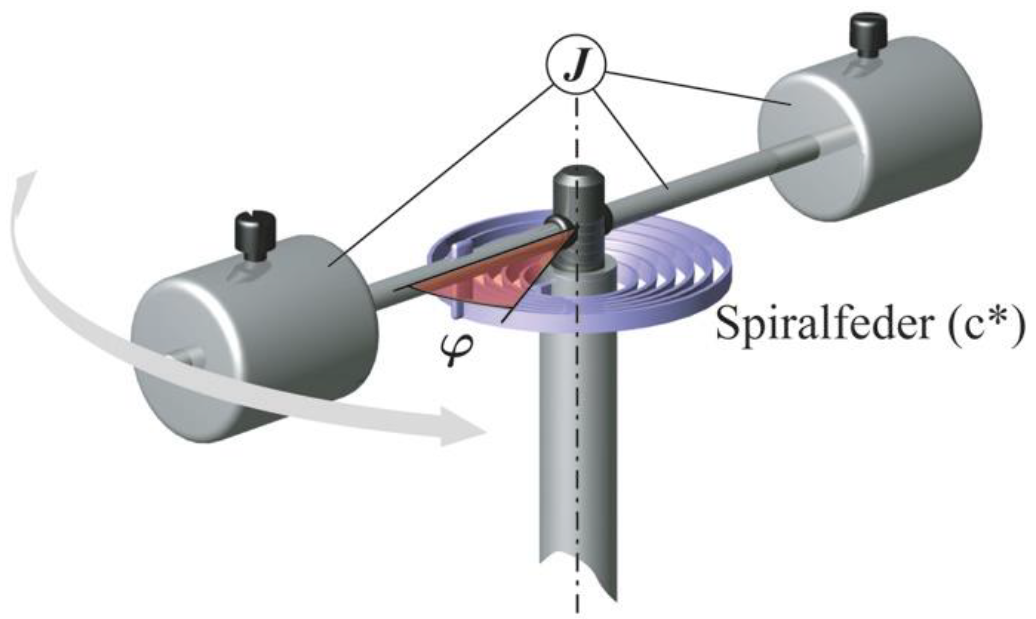
\includegraphics[width=0.9\linewidth]{Bilder/Wellen-Optik/drehpendel}
\end{minipage}
\hfill
\begin{minipage}{0.56\linewidth}

Analogie ohne Rotation: 
\center{ $F = - k \cdot x \qquad F = m \cdot a = m \cdot \ddot{x} $ }\\

\center{ $ M = - c^* \, \varphi \qquad M = J \cdot \ddot{\varphi} $ } 

\center{Gleichgewicht:  $J \cdot \ddot{\varphi} = - c^* \, \varphi $ } 


$$ \boxed{ \text{DGL: } \ddot{\varphi} = - \omega^2 \cdot\varphi \quad \text{mit } \omega^2 = \frac{c^*}{J}  }$$

$\varphi$ folgt der gleichen DGL wie $x$ im Fall des Federpendels \\

\center{ $ \varphi(t) = \varphi_0 \cdot \sin(\omega \, t + \delta) $} \\
\end{minipage}

\vspace{0.2cm}


\begin{tabular}{lll}
$J$ & Trägheitsmoment & $[J] = \kg \cdot \m^2$ \\
\rule{0pt}{15pt}$c^*$ & Winkelrichtgrösse & $[c^*] = \mathrm{\frac{N \, m}{rad}}$ \\
\end{tabular}


\subsubsection{Torsionspendel}
\begin{minipage}{0.3\linewidth}
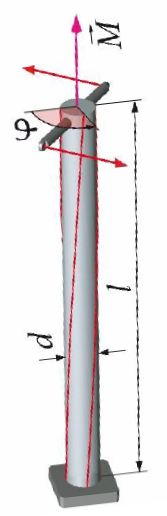
\includegraphics[width=0.5\linewidth]{Bilder/Wellen-Optik/torsionspendel} \\
\end{minipage}
\hfill
\begin{minipage}{0.62\linewidth}

\center{ Variante des Drehpendels mit der Winkelrichtgrösse \\

$$ \boxed{ c^* = \frac{\pi r^4 G}{2l} } $$  


\begin{tabular}{ll}
$G$ & Torsionsmodul \\
$l$ & Länge \\
$r = \frac{d}{2}$ & Radius \\
\end{tabular}

}
\end{minipage}





\subsubsection{Physikalisches Pendel}

\begin{minipage}{0.32\linewidth}
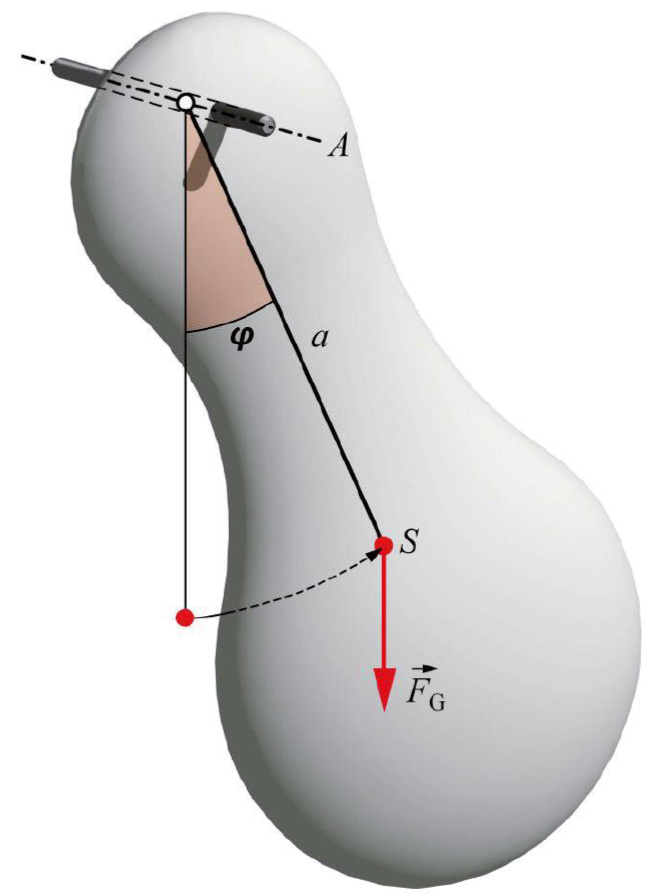
\includegraphics[width=0.98\linewidth]{Bilder/Wellen-Optik/physikalisches_pendel} \\
\end{minipage}
\hfill
\begin{minipage}{0.66\linewidth}

\center{ $ M = - a \cdot \sin(\varphi) \cdot F_G = -a \cdot m \cdot g \cdot  \sin(\varphi) $ }\\

\center{Bewegungsgleichung: $ M = J_A \cdot \ddot{\varphi}$ } 

\center{Gleichgewicht:  $-a \cdot m \cdot g \cdot  \sin(\varphi) =  J_A \cdot \ddot{\varphi} $ } 
\center{Kleine Winkel:  $-a \cdot m \cdot g \cdot \varphi =  J_A \cdot \ddot{\varphi} $ }


$$ \boxed{ \text{DGL: } \ddot{\varphi} = -\omega^2 \, \varphi  \quad \text{mit } \omega^2 =  \frac{g}{L^*} = \frac{g \cdot a \cdot m}{J_A}  }$$

\center{$ \boxed{L^* = \frac{J_A}{a \cdot m}} \qquad \boxed{J_A = J_s + m \cdot a^2 } $  } \\

\vspace{0.2cm}

$\varphi$ folgt der gleichen DGL wie $x$ im Fall des Federpendels \\

\end{minipage}

\textbf{Auch gültig für mehrere Massen:}
$$ \boxed{  T = \frac{2 \, \pi}{\omega} = 2 \, \pi \sqrt{\frac{J_{A1} + J_{A2}}{(a_1 \cdot m_1 + a_2 \cdot m_2) \cdot g}} } $$

$\boldsymbol{ \Rightarrow} $ \textbf{J-Tabelle im Anhang Abschnitt \ref{Massenträgheitsmomente}} \\



\begin{tabular}{lll}
$S$ &  Schwerpunkt des Körpers &  \\
$J_s$ & Trägheitsmoment bzgl. $S$ & $[J_S] = \kg \cdot \m^2$ \\
$a$ & Abstand Schwerpunkt - Drehpunkt & $[a] = \m$ \\
$L^*$ & Reduzierte Länge & $[L^*] = \m$ \\
$J_A$ & Trägheitsmoment um Aufhängepunkt & $[J_A] = \kg \cdot \m^2$ 
\end{tabular}



\subsection{Perkussionszentrum}

\textbf{Frage:} Wie weit vom Drehpunkt $A$ muss ein Impuls auf einen Körper ausgeübt werden, damit keine Kraft auf die Achse ausgeübt wird? \\

\textbf{Antwort:} Auf Höhe der reduzierten Länge $L^* = \frac{J_A}{a \cdot m}$ \\
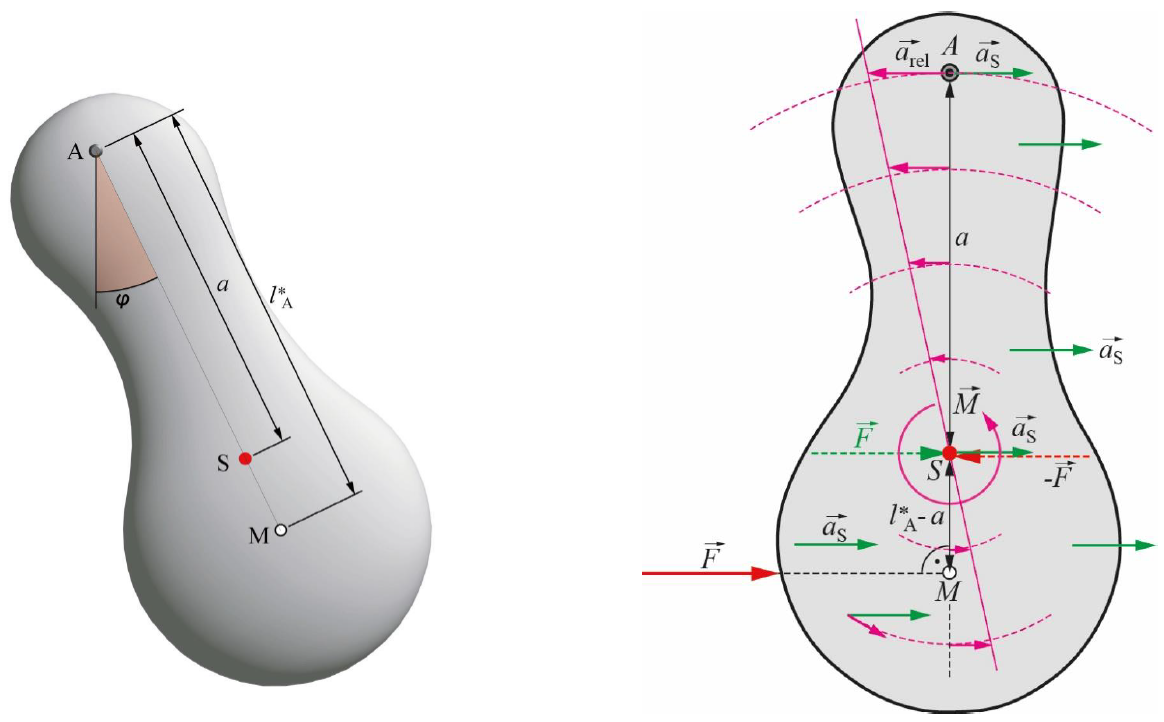
\includegraphics[width=0.8\linewidth]{Bilder/Wellen-Optik/perkussionszentrum} \\


% \vfill\null
% \columnbreak


\subsection{Periodische Schwingung}

\begin{minipage}{0.48\linewidth}
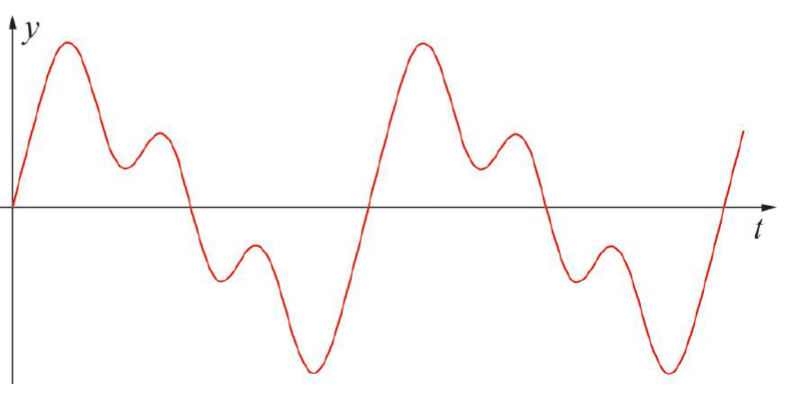
\includegraphics[width=0.8\linewidth]{Bilder/Wellen-Optik/periodische_schwingung} 
\end{minipage}
\hfill
\begin{minipage}{0.48\linewidth}

Muster wiederholt sich 

$$ \boxed{ f(t) = f(t - T ) }$$
\end{minipage}


Periodische Schwingungen können im \textbf{Frequenzbereich} in \\
eine \textbf{Grundschwingung} und \textbf{Oberschwingungen}\\
\textbf{(Harmonische)} zerlegt werden. 

$$ \boxed{ f(t) = A_0 + \sum\limits_{n=1}^{\infty}  A_n \, \sin(n \cdot \omega + \varphi_n)  } $$

\begin{tabular}{ll}
$\omega_0 = \frac{2 \, \pi}{T}$ & Grundschwingung \\
$\omega_n = n \cdot \omega_0$ & n-te Harmonische \\
\end{tabular}



\subsubsection{Fourier-Analyse}

$$ \boxed{ f(t) = A_0 +  \sum\limits_{n=1}^{\infty}  A_n \, \cos  \Big(\frac{ 2 \, \pi \, n}{T} t \Big) + \sum\limits_{n=1}^{\infty}  B_n \, \sin \Big(\frac{ 2 \, \pi \, n}{T} t \Big)  } $$

\begin{minipage}{0.6\linewidth}
\center{ $ A_n = \frac{2}{T} \int\limits_{-T/2}^{T/2} f(t) \, \cos \Big(\frac{ 2 \, \pi \, n \, t}{T}  \Big)  \, dt $}
\end{minipage}
\hfill
\begin{minipage}{0.33\linewidth}
\center{$A_0 = \frac{1}{T} \int\limits_{-T/2}^{T/2} f(t) \, dt $}
\end{minipage}


\begin{minipage}{0.6\linewidth}
\center{ $ B_n = \frac{2}{T} \int\limits_{-T/2}^{T/2} f(t) \, \sin \Big(\frac{ 2 \, \pi \, n \, t}{T}  \Big)  \, dt $}
\end{minipage}
\hfill
\begin{minipage}{0.33\linewidth}

\end{minipage}





\subsection{Signalmodulationen}

$$ \boxed{ x(t) = A \sin ( \omega t + \varphi)} $$ 

\begin{tabular}{ll}
Amplitudenmodulation (AM) & Veränderung von $ A $ \\
Frequenzmodulation (FM) & Veränderung von $ \omega $ \\
\\
\end{tabular}

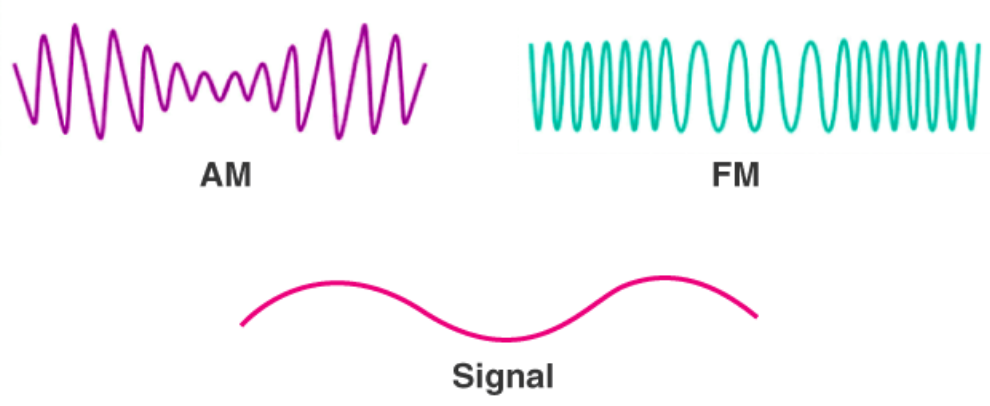
\includegraphics[width=0.65\linewidth]{Bilder/Wellen-Optik/AM_FM}

% \vfill\null
% \columnbreak


\subsection{Gedämpfte Schwingungen}

\subsubsection{Gedämpfte Schwingung - Konstante Reibungskraft}

$$ m \ddot{x}(t) = -k x(t) - \mu F_N \quad \text{für } \ddot{x}(t) > 0 $$

$$ m \ddot{x}(t) = -k x(t) + \mu F_N \quad \text{für } \ddot{x}(t) < 0 $$


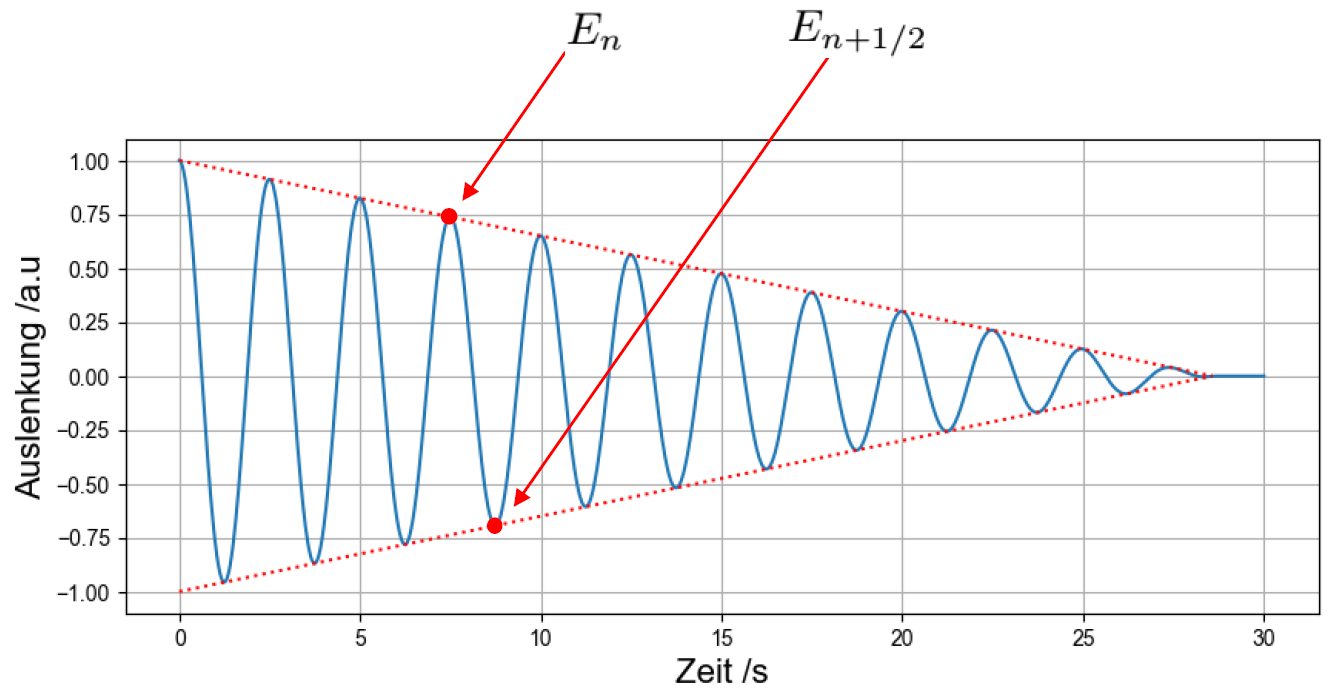
\includegraphics[width=0.7\linewidth]{Bilder/Wellen-Optik/gedaempfte_schwingungen_konst_reibung} 




\begin{minipage}{0.48\linewidth}
$$ \boxed{ E = \frac{k \, A^2}{2} } $$ \\
\end{minipage}
\hfill
\begin{minipage}{0.48\linewidth}
$$ \boxed{ \Delta A = 4 \frac{F_R}{k}} $$ \\
\end{minipage}


\begin{tabular}{c l c}
$E$ & Energie bei max. Auslenkung & $[E] = \J$ \\
$k=c$ & Federkonstante & $[k] = \frac{\N}{\m}$ \\
$A$ & Amplitude bei max. Auslankung & $[A] = \m$ \\
$\Delta A$ & Amplitudenänderung pro Periode & $[\Delta A] = \m$ \\
$F_R$ & Reibungskraft & $[F_R] = \N$ 
\end{tabular}



\subsubsection{Gedämpfte Schwingungen - Dämpfung proportional zur Geschwindigkeit}
$$ \boxed{\ddot{x}(t) + 2\delta \dot{x}(t) + \omega^2x(t) = 0, \quad D = \frac{\delta}{\omega}, \quad f = \frac{\Omega}{2 \, \pi}} $$
\tiny
\setlength{\tabcolsep}{3pt}
\begin{tabular}{|l|c|l|l|}\hline
        1. Fall: & $\delta^2 - \omega^2 > 0$, D $>$ 1 & $ x(t) = A \e^{\lambda_1t} + B\e^{\lambda_2t} $ & Aperiod. Schwingung \\ 
        & & & \\ \hline
        2. Fall: & $\delta^2 - \omega^2 < 0$, D $<$ 1 & $ x(t) = A \e^{-\delta t} cos(\Omega t + \varphi) $ & Period. Schwingung \\
        & & & \\\hline
        3. Fall: & $\delta^2 - \omega^2 = 0$, D $=$ 1 & $ x(t) = (A + Bt)\e^{-\delta t} $ & Grenzfall ($\lambda = -\delta$) \\
        & & & \\\hline
\end{tabular}
\normalsize


% 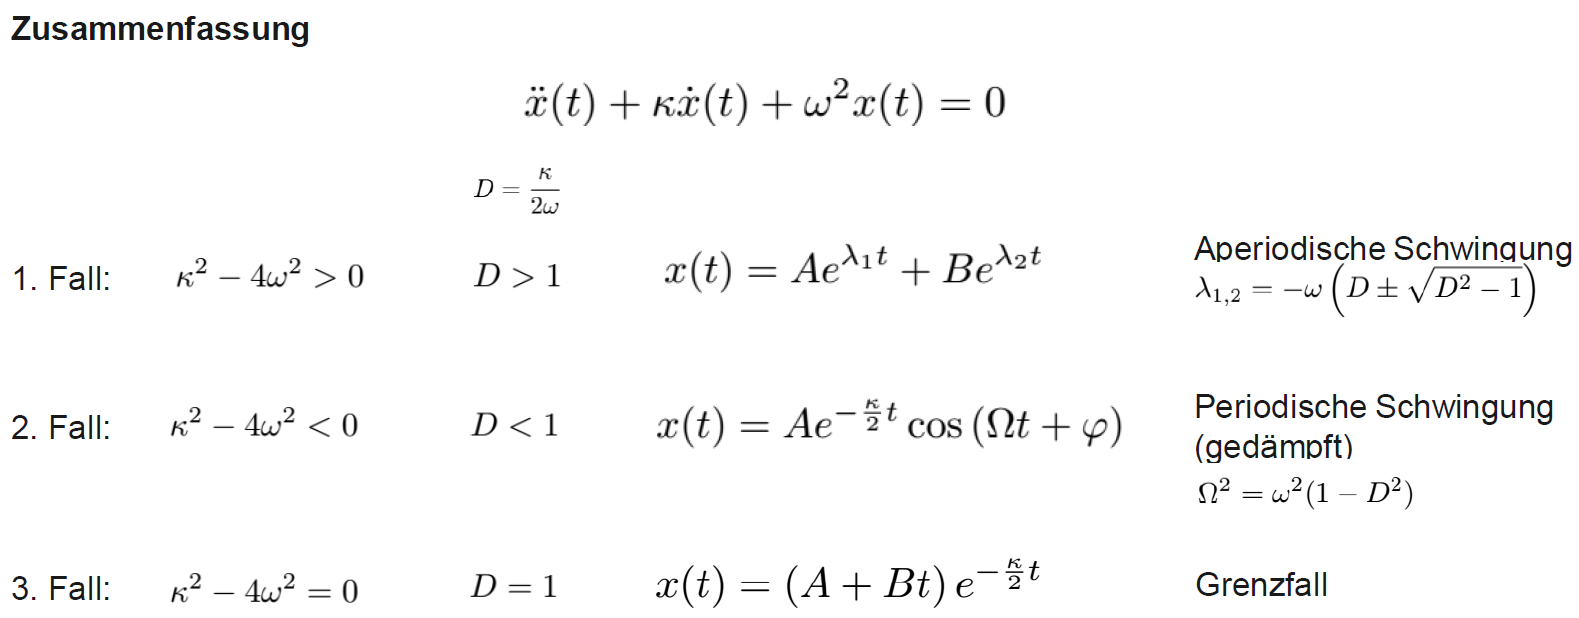
\includegraphics[width=0.98\linewidth]{Bilder/Wellen-Optik/gedaempfte_schwingungen} \\

\begin{minipage}{0.5\linewidth}
    $$ \boxed{ \lambda_{1,2} = -\omega ( D \pm \sqrt{D^2 -1}) }$$ 
    $$ \boxed{ \Omega^2 =  \omega^2 - \delta^2 }$$ 
\end{minipage}
\hfill
\begin{minipage}{0.45\linewidth}
    $$ \boxed{ z \cdot \Lambda = \ln \Big( \frac{A_n}{A_{n+z}} \Big) = z \cdot \delta T }$$ \\
\end{minipage}

\begin{tabular}{c l c}
$\frac{\kappa}{2} = \delta$ & Abklingkonstante & $[\kappa = \delta] = \frac{1}{\s}$ \\
$\omega$ & Kreisfrequenz ungedämpfte Schwingung & $[\omega] = \frac{\rad}{\s}$ \\
$D$ & Dämpfungsgrad & $[D] = 1$ \\
$\Omega$ & Kreisfrequenz gedämpfte Schwingung & $[\Omega] = \frac{\rad}{\s}$ \\


$\Lambda$ & Logarithmisches Dekrement & $[\Lambda] = 1$ \\
$A_n$ & Amplitude zum Zeitpunkt $t$ & $[A_n] = \m$ \\
$A_{n+z}$ & Amplitude zum Zeitpunkt $t + z \cdot T$ & $[A_{n+z}] = \m$ \\
$z$ & Anzahl verstrichene Schwingungen & $[z] = 1$ \\
$T$ & Periodendauer & $[T] = \s$ \\
$f$ & Frequenz der gedämpften Schwingung & $[f] = \Hz$ 
\end{tabular}





\subsection{Fremderregte Schwingung}

\subsubsection{Definition}

Erzwungene Schwingungen sind Schwingungen, die durch eine \\
\textbf{periodische Störung} verursacht werden.



\subsection{Fremderregte Schwingungen - Krafterregung}
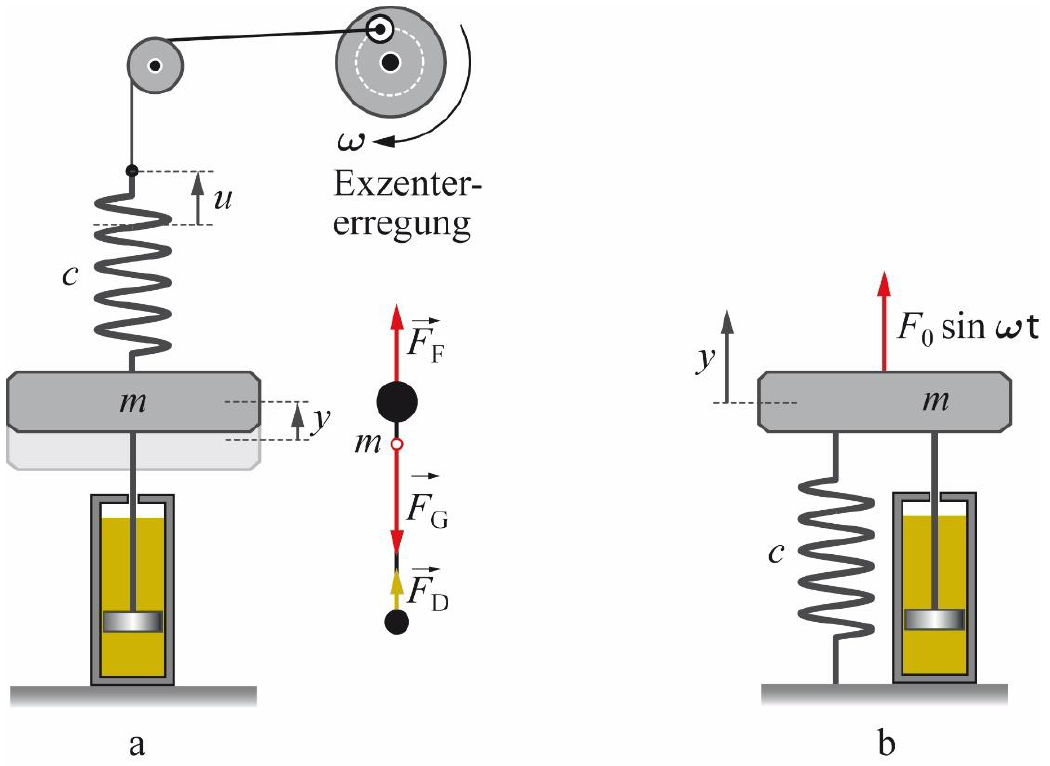
\includegraphics[width=0.75\linewidth]{Bilder/Wellen-Optik/krafterregung} 

$$ \boxed{ \text{DGL: } m \, \ddot{y} + b \, \dot{y} + c \, y = F_0 \, \sin(\omega \, t)  } $$  


$$ y(t) = \underbrace{ A(\omega) \, \sin(\omega \, t - \varphi) }_{\substack{y_p(t)}} + \underbrace{ B \, e^{- \frac{\kappa}{2} t} \sin(\omega_d \, t + \varphi_0)}_{\substack{y_h(t)}} $$

\begin{minipage}{0.3\linewidth}
$$ \boxed{ \varphi = \arctan \Big( \frac{2 D \omega_0 \omega}{\omega_0^2 - \omega^2}   \Big) } $$ \\
\end{minipage}
\hfill
\begin{minipage}{0.68\linewidth}
$$ \boxed{ A(\omega) = \frac{F_0}{m \sqrt{(\omega_0^2- \omega^2)^2 + (2 D \omega_0 \omega)^2 } } }$$ \\
\end{minipage}


\begin{tabular}{c l c}
$A(\omega)$ & Amplitudenverlauf & $[A(\omega)] = \m$ \\
$\varphi$ & Phasenverschiebung & $[\varphi] = \rad$
\end{tabular}



\subsubsection{Übersicht über Hilfsgrössen}

\fbox{\parbox{0.8\linewidth}{

\begin{tabular}{c c c c c}
$\omega_0 = \sqrt{\frac{k}{m}}$ & &  $\delta = \frac{\kappa}{2} = \frac{b}{2 \, m}$ & & $ D = \frac{\delta}{\omega_0} =  \frac{\kappa}{2 \, \omega_0}$\\
\\
\end{tabular}
 
 
\begin{tabular}{c c c}
$\eta = \frac{\omega}{\omega_0}$ & & $\omega_d = \sqrt{\omega_0^2 - \big( \frac{\kappa}{2} \big) ^2} =  \omega_0 \sqrt{1 - D^2}$\\
\end{tabular}
}}

\begin{tabular}{c l c}
\rule{0pt}{10pt} $\omega_0$ & Kreisfrequenz ungedämpfte Schwingung & $[\omega_0] = \frac{\rad}{\s}$ \\
\rule{0pt}{10pt} $\omega_d$ & Kreisfrequenz gedämpfte Eigenfrequenz & $[\omega_d] = \frac{\rad}{\s}$ \\
\rule{0pt}{10pt} $\omega_r$ & Resonanzkreisfrequenz & $[\omega_r] = \frac{\rad}{\s}$ \\
\rule{0pt}{10pt} $\omega$ & Kreisfrequenz der Störung (Erreger) & $[\omega] = \frac{\rad}{\s}$ \\
\rule{0pt}{10pt} $\frac{\kappa}{2}$ & Abklingkonstante & $[\kappa] = \frac{1}{\s}$ \\
\rule{0pt}{10pt} $D$ & Dämpfungsgrad & $[D] = 1$ \\
$\eta$ & Dimensionslose Frequenz & $[\eta] = 1$  \\
$k = c$ & Federkonstante & $[k] = \frac{\N}{\m}$
\end{tabular}


% \vfill\null
% \columnbreak


\subsubsection{Resonanz}

Die Amplitude $A$ wird maximal, wenn der Nenner von $A(\omega)$ minimal wird 

\begin{minipage}{0.48\linewidth}
$$ \boxed{ \omega_r = \omega_0 \sqrt{1 - 2 \, D^2} } $$
\end{minipage}
\hfill
\begin{minipage}{0.48\linewidth}
$$ \boxed{ A_r = \frac{u_0}{2 \, D \sqrt{1 - D^2}} }$$
\end{minipage}


\subsubsection{Vergrösserungsfunktion / Phasenverschiebung}

\begin{tabular}{c c}
$ \boxed{ V = \frac{1}{\sqrt{(1- \eta^2)^2 + (2 \, D \, \eta)^2} } } $ & $ \boxed{ \varphi = \arctan \Big( \frac{2 D \eta}{1 - \eta^2}  \Big) } $ \\
\\
$ \boxed{ V_r = \frac{1}{\sqrt{ 1 - \eta_r^4} } \quad \text{mit } \eta_r = \sqrt{1 - 2 \, D^2}  } $ \\
\\
\end{tabular}


\begin{tabular}{c l c}
$\varphi$ & Phasenverschiebung & $[ \varphi] = \rad$ \\
$V$ & Vergrösserungsfunktion & $[V] = 1$ \\
$V_r$ & Vergrösserungsfunktion & $[V_r] = 1$ \\
$\eta$ & Dimensionslose Frequenz & $[\eta] = 1$  \\
$D$ & Dämpfungsgrad & $[D] = 1$ 
\end{tabular}




\subsection{Fremderregte Schwingungen - Dämpfererregung}

\begin{minipage}{0.25\linewidth}
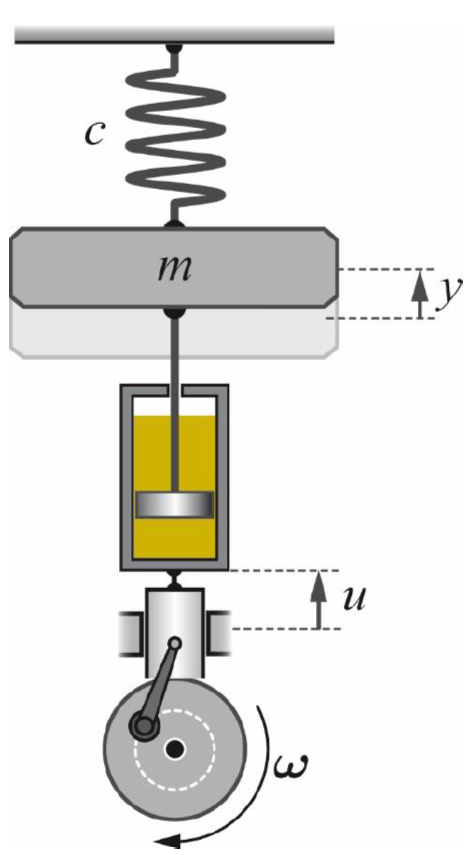
\includegraphics[width=0.9\linewidth]{Bilder/Wellen-Optik/daempfererregung} \\
\\
\end{minipage}
\hfill
\begin{minipage}{0.72\linewidth}
$$ \boxed{ \text{DGL: } m \, \ddot{y} + b \, \dot{y} + c \, y = b \, \omega  \, u_0 \, \cos(\omega \, t)  } $$  

$$ A(\omega) =  \frac{b \, \omega \, u_0}{\sqrt{(\omega_0^2 -\omega^2)^2 + (2D \omega_0 \omega)^2}} $$ 

$$ \boxed{ V = \frac{2 \, D \, \eta}{\sqrt{(1- \eta^2)^2 + (2 \, D \, \eta)^2} } } $$

$$ \boxed{ \varphi = \arctan \Big( \frac{2 D \eta}{1 - \eta^2} \Big) - \frac{\pi}{2} } $$ 


\end{minipage}


\begin{tabular}{c l c}
$A(\omega)$ & Amplitude der Schwingung & $[A(\omega)] = \m$ \\
$\varphi$ & Phasenverschiebung & $[ \varphi] = \rad$ \\
$V$ & Vergrösserungsfunktion & $[V] = 1$ \\
$\eta$ & Dimensionslose Frequenz & $[\eta] = 1$  \\
$D$ & Dämpfungsgrad & $[D] = 1$ \\
\end{tabular}

% \vfill\null
% \columnbreak



\subsection{Fremderregte Schwingungen - Stützenerregung}

$$ \boxed{ \text{DGL: } m \, \ddot{q} + b \, \dot{q} + c \, q = -m \, \omega^2 \, u_0 \, \sin(\omega \, t)  \quad \text{mit } q = y - u } $$

\begin{minipage}{0.25\linewidth}
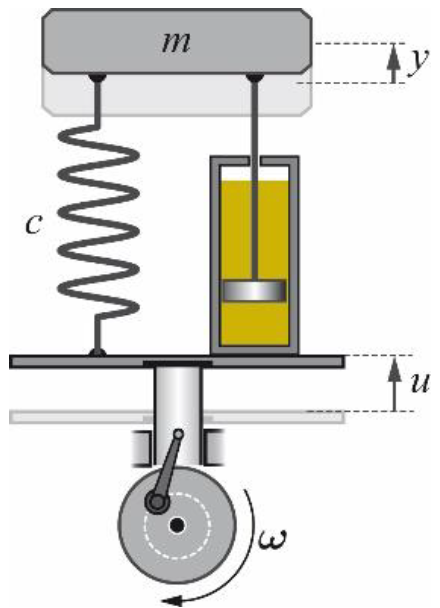
\includegraphics[width=0.9\linewidth]{Bilder/Wellen-Optik/stuetzenerregung} 
\end{minipage}
\hfill
\begin{minipage}{0.72\linewidth}
$$ A(\omega) = \frac{\omega^2 u_0}{\sqrt{(\omega_0^2 -\omega^2)^2 + (2D \omega_0 \omega)^2}} $$ 
\end{minipage}

\begin{minipage}{0.48\linewidth}
$$ \boxed{ V = \frac{\eta^2}{\sqrt{(1- \eta^2)^2 + (2 \, D \, \eta)^2} } } $$
\end{minipage}
\hfill
\begin{minipage}{0.48\linewidth}
$$ \boxed{ \varphi = \arctan \Big( \frac{2 D \eta}{1 - \eta^2} \Big) - \pi } $$ 
\end{minipage}

\vspace{0.2cm}

\begin{tabular}{c l c}
$\varphi$ & Phasenverschiebung & $[ \varphi] = \rad$ \\
$V$ & Vergrösserungsfunktion & $[V] = 1$ \\
$\eta$ & Dimensionslose Frequenz & $[\eta] = 1$  \\
$D$ & Dämpfungsgrad & $[D] = 1$  \\
\rule{0pt}{10pt} $\omega_0$ & Kreisfrequenz ungedämpfte Schwingung & $[\omega_0] = \frac{\rad}{\s}$ \\
\rule{0pt}{10pt} $\omega$ & Kreisfrequenz der Störung (Erreger) & $[\omega] = \frac{\rad}{\s}$ \\
$A(\omega)$ & Amplitude der Schwingung & $[A(\omega)] = \m$
\end{tabular}



\subsection{Fremderregte Schwingung - Unwuchterregung}
\textbf{Unwucht:} Schwerpunkt $S$ des Rotors der Masse $m_R$ bewegt sich auf einem Kreis mit Radius $e$ \\

\begin{minipage}{0.52\linewidth}
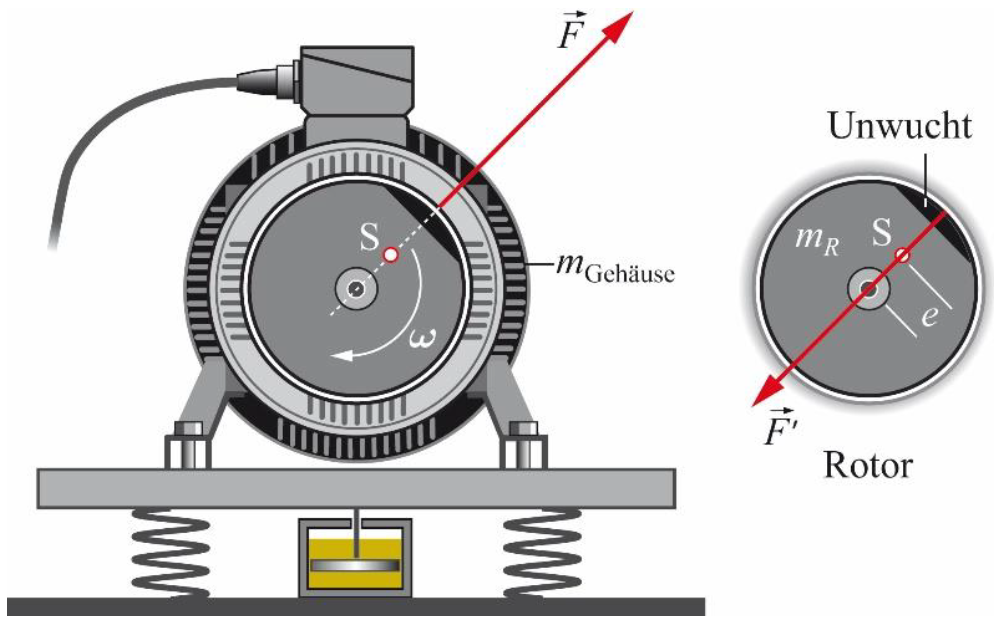
\includegraphics[width=0.9\linewidth]{Bilder/Wellen-Optik/unwucht} \\
\end{minipage}
\hfill
\begin{minipage}{0.44\linewidth}
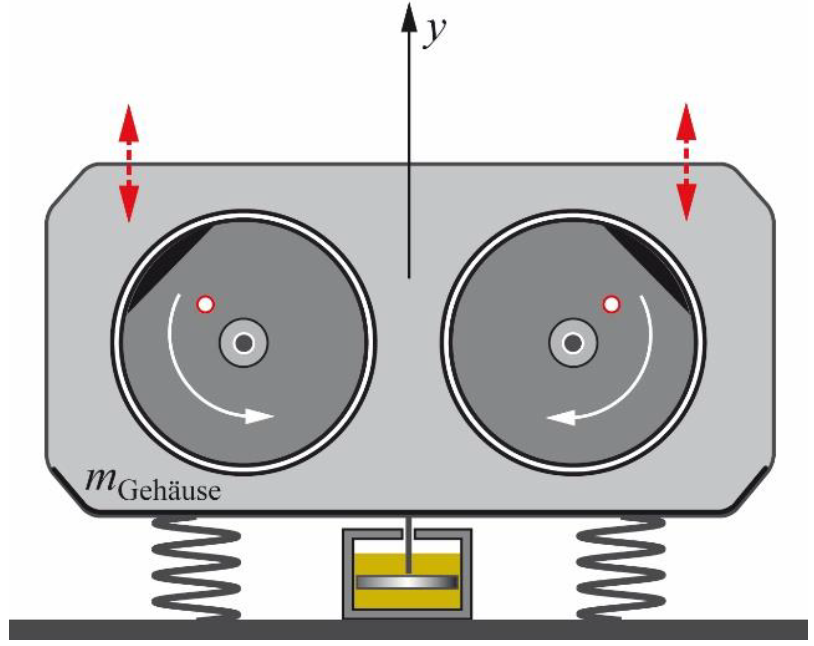
\includegraphics[width=0.89\linewidth]{Bilder/Wellen-Optik/unwucht_gehause} \\
\end{minipage}

$$ \boxed{ \text{DGL in y-Richtung: } m \ddot{y} + b \dot{y} + c \, y = -m_R \, \omega^2 \, \sin(\omega \, t) }  $$

Radiale Beschleunigung des Schwerpunkts des Rotors: $a_R = \omega^2 e$ \\

Kraft des Rotors auf die Maschine: $\boxed{ F_U = m_R \cdot a_R = m_R \cdot \omega^2 e } $ 

$$ A(\omega) = \frac{m_R}{m} \frac{e \, \omega^2}{\sqrt{(\omega_0^2 -\omega^2)^2 + (2D \omega_0 \omega)^2}}  $$ 


$$ A_R = \frac{m_R}{m} \frac{e}{2D \sqrt{1 - D^2}}  $$


% \vfill\null
% \columnbreak


\subsubsection{Kraft auf die Basis des Gehäuses} 

\begin{minipage}{0.48\linewidth}
$$ F_B = c y + b \dot{y} = F_{B0} \sin(\omega t - \varphi + \psi) $$ 
\end{minipage}
\hfill
\begin{minipage}{0.48\linewidth}
$$\boxed{ F_{B0} = \frac{m_R \, e \, \omega^2 \sqrt{1+ (2D \eta)^2}}{\sqrt{(1 - \eta^2)^2 + (2 D \eta)^2}} } $$ 
\end{minipage}
\vspace{0.2cm}


\begin{tabular}{c l c}
$m_R$ & Masse des Rotors & $[m_R] = \kg$ \\
$a_R$ & Radiale Beschleinigung Schwerpunkt & $[a_R] = \frac{\m}{\s}$ \\
$e$ & Abstand Mittelpunkt - Schwerpunkt & $[e] = \m$ \\
$\varphi$ & Phasenverschiebung & $[ \varphi] = \rad$ \\
$V$ & Vergrösserungsfunktion & $[V] = 1$ \\
$\eta$ & Dimensionslose Frequenz & $[\eta] = 1$  \\
$D$ & Dämpfungsgrad & $[D] = 1$  \\
$A(\omega)$ & Amplitude & $[A(\omega)] = \m$ \\
$A_R$ & Resonanzamplitude & $[A_R] = \m$
\end{tabular}




\subsection{Fremderregte Schwingung - Schwingkereis}

\begin{minipage}{0.3\linewidth}
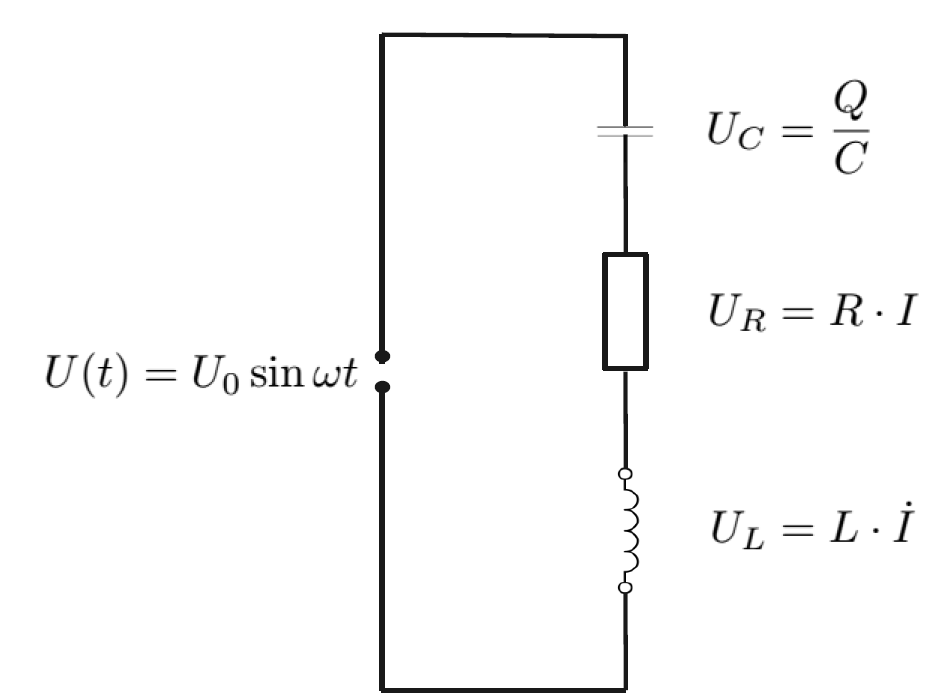
\includegraphics[width=\linewidth]{Bilder/Wellen-Optik/schwingkreis}  \\
\end{minipage}
\hfill
\begin{minipage}{0.68\linewidth}
$$ \boxed{ \text{DGL: } L \ddot{I} + R \dot{I} + \frac{1}{C} \, I = \omega \, U_0 \,\sin(\omega \, t + \frac{\pi}{2}) } $$

$\Rightarrow$ Gleiche DGL wie bei \textcolor{blue}{Dämpfererregung} \\
\end{minipage}


$ \textcolor{blue}{\text{DGL: } m \ddot{y} + b \dot{y} + c \, y = b \, \omega \, u_0 \, \cos(\omega \, t) } $
\quad
$ \textcolor{blue}{A(\omega) =  \frac{b \, \omega \, u_0}{\sqrt{(\omega_0^2 -\omega^2)^2 + (2D \omega_0 \omega)^2}} } $ \\

\vspace{0.1cm}


$ \boxed{ I(\omega) =  \frac{\omega}{\sqrt{(\omega_0^2 -\omega^2)^2 + (2D \omega_0 \omega)^2}}U_0  \text{  mit }\omega_0 = \frac{1}{\sqrt{LC}} , \, D = \frac{R}{2}\sqrt{\frac{C}{L}}} $ 

\vspace{0.1cm}

$$ \boxed{ V = \frac{U_{L0}}{U_0} = \frac{\eta^2}{\sqrt{(1 - \eta^2)^2 + (2 \, D \, \eta)^2}} }$$



\subsubsection{Resonanz}

\begin{minipage}{0.48\linewidth}
\textbf{Resonanzfrequenz}
$$ \boxed{ \omega_r = \omega_0 = \frac{1}{\sqrt{LC}} } $$ 
\end{minipage}
\hfill
\begin{minipage}{0.48\linewidth}
\textbf{Amplitude @ Resonanz}
$$ \boxed{ I_{0r} = \frac{U_0}{R} } $$ 
\end{minipage}


\vspace{0.2cm}


\begin{tabular}{c l c}
\rule{0pt}{10pt} $\omega_0$ & Kreisfrequenz ungedämpfte Schwingung & $[\omega_0] = \frac{\rad}{\s}$ \\
\rule{0pt}{10pt} $\omega$ & Kreisfrequenz der Störung (Erreger) & $[\omega] = \frac{\rad}{\s}$ \\
\rule{0pt}{10pt} $\omega_r$ & Resonanzfrequenz & $[\omega_r] = \frac{\rad}{\s}$ \\
$I_{0r}$ & Strom-Amplitude @ Resonanz & $[I_{0r}] = \A$ \\
$U_0$ & Amplitude der Erregerspannung & $[U_0] = \V$ \\
$U_{L0}$ & Amplitude Spulenspannung & $[U_{L0}] = \V$ \\
$A(\omega)$ & Amplitude der Schwingung & $[A(\omega)] = \m$ \\
$V$ & Vergrösserungsfunktion & $[V] = 1$ \\
$\eta$ & Dimensionslose Frequenz & $[\eta] = 1$  \\
$D$ & Dämpfungsgrad & $[D] = 1$ 
\end{tabular}





\subsection{Fremderregte Schwingung - Güte $Q$}
\subsubsection{Definition}

Die relative Abnahme der Schwingungsenergie $E(t)$ pro Schwingdauer wird als \textbf{Güte} oder \textbf{Gütefaktor} bezeichnet 

$$ \boxed{ Q = 2 \pi \frac{E(t)}{E(t) - E(t + T)} }$$ 



\subsubsection{Beziehungen}

\begin{minipage}{0.4\linewidth}
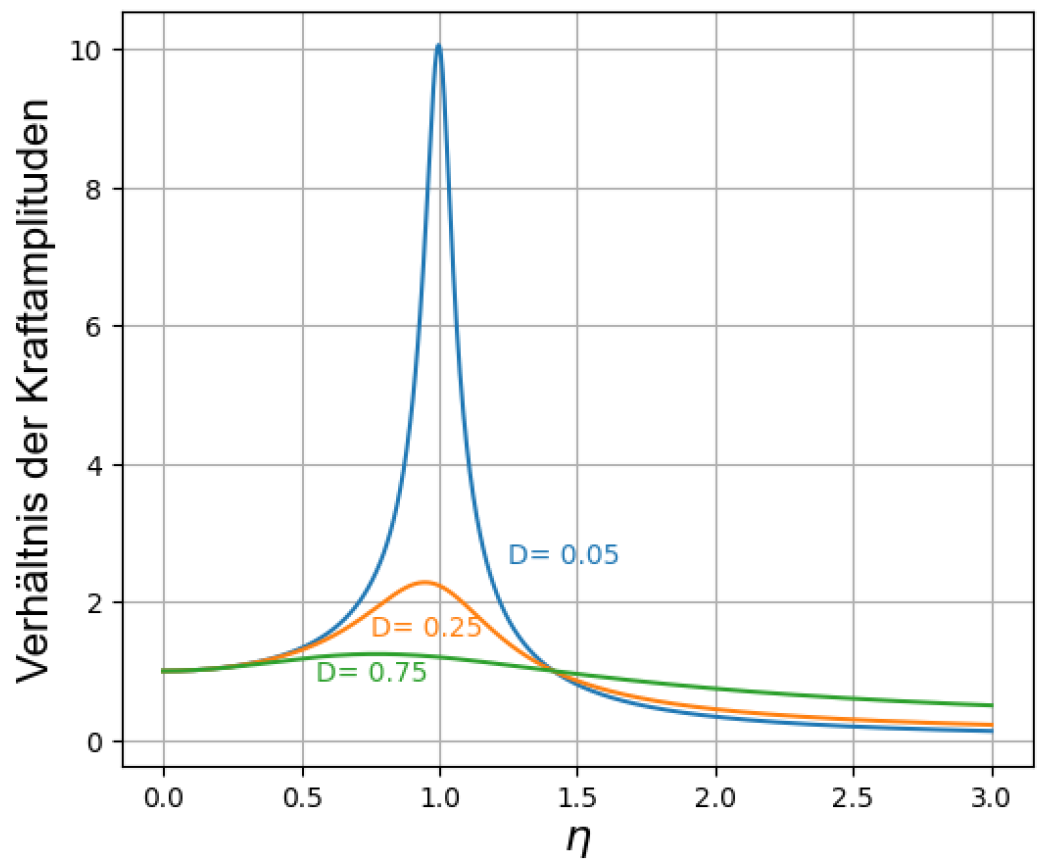
\includegraphics[width=0.95\linewidth]{Bilder/Wellen-Optik/guete_resonanz} 
\end{minipage}
\hfill
\begin{minipage}{0.58\linewidth}

\begin{minipage}{0.48\linewidth}
$$ \boxed{Q = \frac{1}{2 \, D} } $$ 
\end{minipage}
\hfill
\begin{minipage}{0.48\linewidth}
$$ \boxed{ Q = \frac{\omega_0}{\Delta \omega} } $$
\end{minipage}

\vspace{0.2cm}

Breite der Resonanzkurve bei $U_0 = \frac{U_{0r}}{\sqrt{2}}$ \\


\textbf{Breite Kurve $\Rightarrow$ tiefe Güte}
\end{minipage}



\subsection{Gekoppelte Pendel}
Zwei Pendel sind durch eine Feder miteinander verbunden. \\
\textbf{Die Bewegung eines Pendels hat Auswirkungen auf die \\
Bewegung des anderen Pendles.} \\
Gesucht ist eine Berschreibung der Bewegung des Pendels. \\

\begin{minipage}{0.3\linewidth}
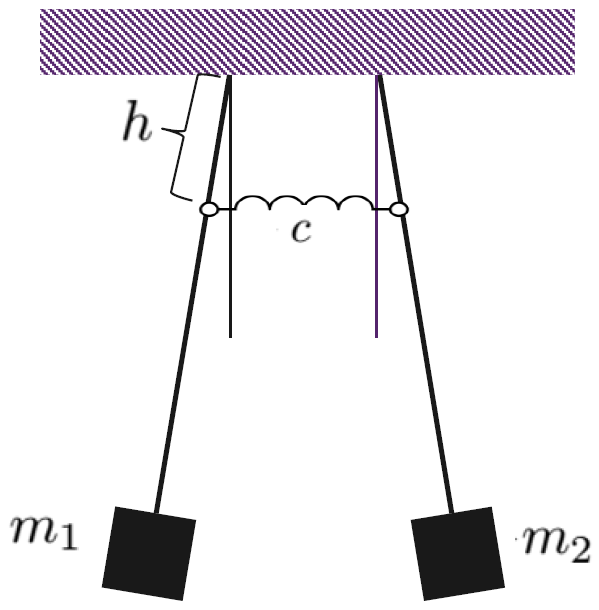
\includegraphics[width=0.95\linewidth]{Bilder/Wellen-Optik/gekoppelte_pendel} 
\end{minipage}
\hfill
\begin{minipage}{0.66\linewidth}
$ J_1 \ddot{\varphi_1} = -m_1 \, g \, a_1 \, \varphi_1 + c \cdot h2 \, (\varphi_2 - \varphi_1)$ \\
$ J_2 \ddot{\varphi_2} = -m_2 \, g \,  a_2 \, \varphi_2 + c \cdot h^2 \, (\varphi_2 - \varphi_1)$ \\

\vspace{0.2cm}

\textbf{Spezialfall $J_1 = J_2 = J$ und $m_1 = m_2 = m$} \\

$ \ddot{\varphi_1} = - \omega^2 \varphi_1 + k \, (\varphi_2 - \varphi_1)$ \\
$ \ddot{\varphi_2} = - \omega^2 \varphi_2 - k \, (\varphi_2 - \varphi_1)$ \\

\vspace{0.2cm}
mit $\Phi_+ = \varphi_1 + \varphi_2$ \qquad $\Phi_- = \varphi_2 + \varphi_1$ \\

$ \omega^2 = \frac{mg}{J}$ \qquad $k = \frac{c \cdot h}{J}$ \qquad $\omega_k = \sqrt{\omega^2 + 2 \, k}$ \\
\end{minipage}


\begin{tabular}{lll}
Symm: & $\ddot{\Phi_+} = - \omega^2 \Phi_+ $ &  $\varphi_1(t) = \varphi_2(t) = \frac{\Phi_0}{2} \cos{ \omega t} $\\
Antisymm: & $\ddot{\Phi_-} = - (\omega^2 + 2k) \Phi_- $ & $\varphi_1(t) = -\varphi_2(t) = \frac{\Phi_0}{2} \cos{ \omega_k t} $ \\
\\
\end{tabular}





\textbf{Allgemeine Lösunge des gekoppelten Systems:} \\
Lineare Kombination der symmetrischen und asymmetrischen Lösung \\

\renewcommand{\arraystretch}{1.3}
\begin{tabular}{lll}
$\varphi_1(t) = \Phi \, \sin( \Omega\, t) \cdot \cos(\overline{\omega} \, t)$ & & $\Omega = \frac{\omega_k - \omega}{2}$ \\
$\varphi_2(t) = \Phi \, \cos( \Omega\, t) \cdot \sin(\overline{\omega} \, t)$ & & $\overline{\omega} = \frac{\omega + \omega_k}{2}$ \\
\\
\end{tabular}
\renewcommand{\arraystretch}{1}


\begin{tabular}{c l c}
$k$ & Kopplungsfaktor & $[k] = 1$ \\
$h$ & Abstand zur Aufhängung & $[h] = \m$ \\
$J$ & Massenträgheitsmoment & $[J] = \kg \cdot \m^2 $ \\
$c$ & Federkonstante & $[c] = \frac{\N}{\m}$ \\
\end{tabular}


% \vfill\null
% \columnbreak